% !TEX root = ./thesis.tex

\chapter{Orthogonal Luciferase−Luciferin Pairs for Bioluminescence Imaging}
\section{Introduction}
Bioluminescence imaging is a popular method for visualizing
cells and other biological features in vivo.\cite{RN26} This technology
relies on enzymes (luciferases) that catalyze the oxidation of
small-molecule substrates (luciferins). The oxidation process is
accompanied by the release of light (Figure \ref{fig:overview}A).
\begin{figure}[htbp]
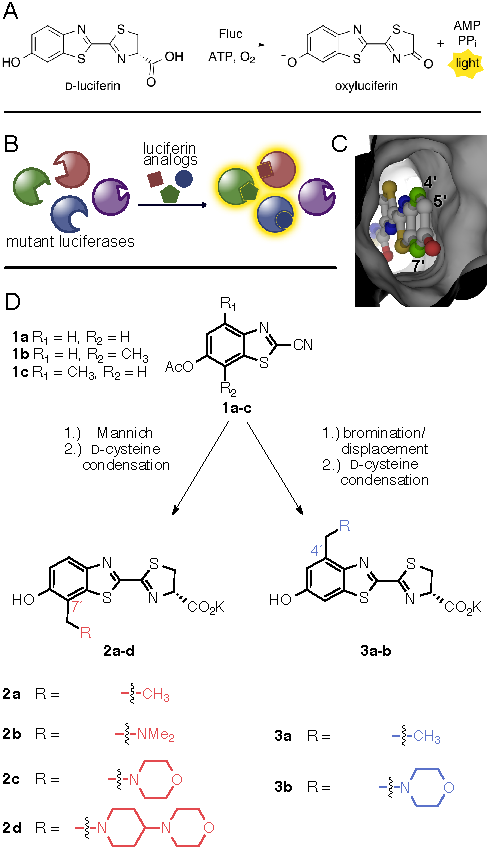
\includegraphics[width=85 mm]{chapter2/fig1}
\centering
\caption[Expanding the bioluminescence toolkit with unique
enzyme−substrate pairs]{Expanding the bioluminescence toolkit with unique
enzyme−substrate pairs. (A) Luciferase-mediated light production
proceeds via an adenylation−oxidation sequence. (B) Strategy to
develop orthogonal luciferase−luciferin pairs via substrate resolution.
Genetically engineered luciferases and chemically modified luciferins
were screened to identify novel partners. Only complementary
enzyme−substrate pairs interact to produce light. (C) Model of \dluciferin{}
bound to firefly luciferase (Fluc). (D) Synthesis of C7′ (left)
and C4′ (right) sterically modified luciferins.}
  \label{fig:overview}
\end{figure}
Since
mammalian cells and tissues do not emit substantial numbers
of photons, bioluminescent light can facilitate sensitive imaging
in these environments.\cite{Prescher:2010dv} Luciferase-labeled cells can also be
imaged repeatedly and noninvasively in a variety of preclinical
models. This broad dynamic range has enabled numerous
studies of fundamental biological processes, including cell
homing and differentiation, proliferation, and cell-to-cell
communication, in physiologically relevant environments.\cite{Badr:2011if}
\par
While versatile, bioluminescence to date has been largely
limited to monitoring one cell type or biological feature at a
time. This is due, in part, to a lack of distinguishable luciferase−
luciferin pairs for in vivo use. The optimal luciferases (from the
insect family) use the same substrate, \dluciferin{}.\cite{RN26,RN101} Thus, they
cannot easily discriminate multiple cell types in a single subject.
Additionally, unlike fluorescent protein technologies, a diverse
suite of accessible bioluminescent probes does not yet exist. To
address this void, \dluciferin{} analogues have been engineered to
emit different colors of light.\cite{RN14,Jathoul:2014do,RN165} However, these substrates are
still utilized by the same luciferases, precluding the distinct
genetic tagging of individual cell types. Insect luciferases have
also been engineered to emit different colors of light with \dluciferin{}.\cite{Branchini:2007fza,Branchini:2007bw,Mezzanotte:2010fq}
The observed emission spectra are not sufficiently
resolved, though, for routine use in complex tissues or animals.
Discriminating among different wavelengths in bioluminescence
(and whole-body optical imaging, in general) is
exceedingly difficult.
\par
Contrasting with these attempts to achieve spectral
resolution, we aimed to obtain distinguishable bioluminescent
probes via substrate resolution. Substrate-resolved bioluminescence
is well precedented in nature, as structurally distinct
luciferase−luciferin pairs have been identified across diverse
phyla.\cite{Haddock:2010cx, Oba:2014cc, RN45} Some of these pairs, including those from the firefly
and Renilla reniformis, have been used extensively.\cite{RN26, Badr:2011if, Porterfield:2015bu, Massoud:2007en} Firefly
(Fluc) and Renilla luciferase employ chemically unique
substrates (\dluciferin{} and coelenterazine, respectively), enabling
their tandem application in vivo.\cite{Bhaumik:2002hf, Maguire:2013kb} Coelenterazine is
less ideal for use in these environments, though, owing to its
suboptimal bioavailability and stability.\cite{RN26, Pichler:2004ke} Other naturally
occurring luciferases and luciferins can be used in combination
with Fluc/\dluciferin{} or other bioluminescent systems.\cite{Maguire:2013kb, Petushkov:2014ha}
However, most of these native pairs remain poorly characterized
or ill-suited for routine use.
\par
Artificial (i.e., mutant) luciferases can exhibit altered
bioluminescent properties, including tolerance for chemically
modified substrates. Fluc itself has been manipulated to process
analogues of \dluciferin{}.\cite{RN98} In elegant work along these lines,
Miller and co-workers prepared a class of non-natural
aminoluciferins that were found to be robust light emitters
with Fluc, but the products inhibited the enzymatic reaction.\cite{Reddy:2010gaa}
Product inhibition was relieved using mutated versions of the
enzyme.\cite{Harwood:2011gl} These same mutations also resulted in sharply
reduced emission with \dluciferin{}, providing key precedent for
the development and utilization of orthogonal pairs.\cite{AdamsJr:2016bn} The
mutant enzymes from these studies, though, were less selective
for one analogue over another perhaps due to the structural
similarities between the luciferin scaffolds. Simultaneous enzyme−substrate manipulation has also been applied to
aequorin (a marine photoprotein) and the luciferase from the
deep-sea shrimp Oplophorus gracilirostris.\cite{Rowe:2009bd,Hall:2012cda} In both cases,
altered bioluminescent outputs (e.g., colors and stabilities) were
achieved, but orthogonal substrate usage was not realized.
\par
Here, we report a strategy for the de novo production of
orthogonal luciferase−luciferin pairs. We synthesized a series of
sterically modified luciferins that were poor emitters with Fluc
but intrinsically capable of robust light production. We then
iteratively screened these analogues with libraries of mutant
luciferases and identified substrate-selective enzymes. The
“hits” were also biochemically characterized. Importantly,
when the mutants and analogues were combined, robust light
production was observed when complementary enzyme−
substrate partners interacted. Sequential administration of
substrates enabled unique luciferases to be illuminated (and
thus resolved) within cultured cell models. These tools promise
to enable a variety of multicellular imaging applications.
Importantly, our approach to identifying orthogonal bioluminescence
pairs is also general and should enable rapid
diversification of the bioluminescence toolkit.

\section{Results and Discussion}

\subsection*{Designing and constructing sterically modified luciferins}
To expediently identify orthogonal bioluminescence
tools, we aimed to screen sterically perturbed luciferins
against libraries of mutant luciferases (Figure \ref{fig:overview}B). We used the
Fluc/\dluciferin{} pair as a starting point for several reasons. First,
this duo is the most widely used in biomedical imaging
applications owing to the nontoxicity of the reagents and
bioavailability of the substrate.\cite{Berger:2008eq, Contag:1997kh} Second, the Fluc/\dluciferin{}
reaction releases the highest percentage of tissue-penetrating
light among known bioluminescent families.\cite{Zhao:2005if} Thus, new
enzymes and substrates based on the firefly pair would be more
applicable to in vivo studies. Third, a wealth of structural and
biochemical information on Fluc could guide our engineering
efforts.\cite{RN45, BRANCHINI:2001gr, Branchini:2003kt, RN107, RN86} Finally, \dluciferin{} derivatives are arguably the
most synthetically tractable luciferin architectures.\cite{Meroni:2009tu, RN172}
\par
Generating an expanded set of bioluminescent tools required
access to diverse luciferin scaffolds. A variety of \dluciferin{}
analogues have been synthesized over the past four
decades,\cite{RN14,RN165,RN112,White:1966gs,Woodroofe:2012vx,McCutcheon:2012ixb,RN100} and those capable of robust emission with
Fluc harbor common features: an electron-donating group at
the 6′ position, a carboxylate appendage (for adenylation), and
an abstractable proton $\alpha{}$ to the carboxylate.\cite{White:1966gs, Branchini:2015epa} Beyond these
requirements, Fluc can tolerate a surprisingly large variety of
modified luciferins,\cite{Meroni:2009ec, White:1966ig, SELIGER:1961dla} including 6′-amino substituents,\cite{RN98, Reddy:2010gaa, White:1966ig}
alkylated\cite{RN99, Wang:2017bc, RN31} and acylated\cite{Kuchimaru:2016eb} scaffolds, and even
luciferins with non-natural chromophores.\cite{Kuchimaru:2016eb, Jathoul:2014do} Crystallographic
analyses have also corroborated these experimental results,
indicating flexibility within the luciferase active site and “space”
to accommodate luciferins with appendages at or near the 6′
position.\cite{RN107, RN86}
\par
Unlike most efforts to produce luciferin analogues reported
to date, we were attracted to the 4′ and 7′ positions of the
luciferin core. These positions lie in close proximity to the Fluc
backbone (Figure \ref{fig:overview}C). Substrates with additional steric bulk at
these sites would likely be occluded from the Fluc active site
and thus good targets for orthogonal probe development: while
poor emitters with the native enzyme, the molecules could
potentially give off light with designer mutants. Indeed,
preliminary docking studies suggested that only analogues
with small (e.g., 2−3 atoms) substituents at C4′ and C7′ could
effectively access the active site.
\par
Generating 4′- and 7′-modified luciferins presented an early
challenge. These positions have been rarely exploited for
analogue development, and no prior syntheses were amenable
to preparing libraries or large quantities of these probes. Rapid,
high-yielding syntheses were essential, as large quantities of
luciferins are required for light emission assays. Fortunately, the
core benzothiazole unit (\cmpd{1a−c}) of the desired analogues could
be accessed from a common route (Figure \ref{fig:overview}D) and in
multigram quantities.\cite{McCutcheon:2012ixb,RN172} From this single intermediate, we
envisioned installing functional handles at C4′ and C7′ to
rapidly assemble a variety of luciferins. We were initially drawn
to an aldehyde group, owing to its ease of diversification under
mild conditions (e.g., reductive amination) and broad
compatibility. Aldehyde installation on \cmpd{1a} was problematic,
though, due to formation of a hydrated hemiacetal.\cite{Jones:1981cm} To circumvent this issue, we turned to more reactive
iminium ions. These electrophiles can be readily trapped by
electron-rich aromatics in a Mannich-type reaction.\cite{Phillips:1956fo} Toward this end, benzothiazole \cmpd{1a} was modified with a series of tertiary
benzyl amines via in situ iminium formation and coupling
(Figure \ref{fig:overview}D and Schemes S2 and S3). The amino appendages
were selected to enhance the water solubility of the luciferin
core. Importantly, this synthetic approach was modular and
amenable to large-scale (1−10 g) syntheses. “Matched” probes
with steric modifications at C4′ were also prepared (\cmpd{3a}, \cmpd{b}). A
different synthetic approach was necessary, though, as the 4′
position cannot be selectively targeted with electrophiles
(Figure \ref{fig:overview}D and Scheme S4).

\subsection*{Analyzing bioluminescent light emission with modified luciferins}

With the modified luciferins in hand, we first
evaluated their optical properties with Fluc. All analogues were
competent light emitters and could be processed by the enzyme
(Figures \ref{fig:chemilum_biolum}A).
\begin{figure}[htbp]
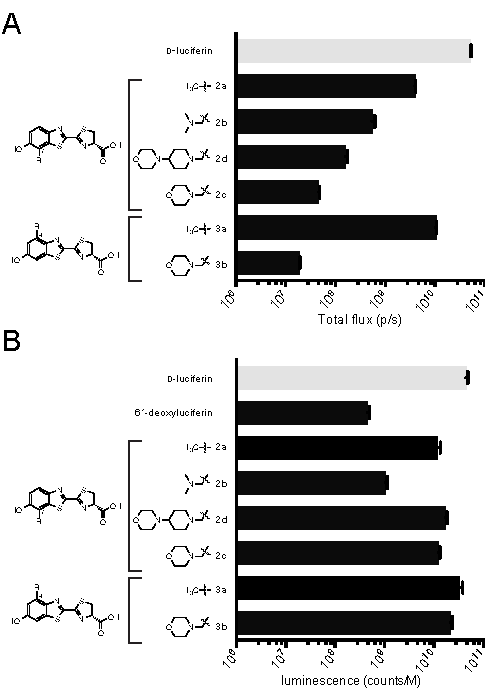
\includegraphics[width=85 mm]{chapter2/fig2}
\centering
\caption[Measuring luciferin light emission]{Measuring luciferin light emission. (A) Bioluminescence
from luciferin analogues (100 μM) incubated with 1 μg of Fluc.
Emission intensities are plotted as total photon flux values on a log
scale. Error bars represent the standard deviation of the mean for n ≥ 3
experiments. (B) Chemiluminescence with luciferin analogues.
Emission intensities are plotted as counts per molar luciferin on a
log scale. Error bars represent the standard error of the mean for n ≥ 3
experiments.}
  \label{fig:chemilum_biolum}
\end{figure}
However, the emission intensities were much weaker than those observed with \dluciferin{}, the native
substrate. Interestingly, the largest analogue (\cmpd{2d}) was not the
weakest emitter, suggesting that steric modification alone does
not dictate luciferin utilization. Similar trends in light emission
were observed across a range of physiological pH values
(Scheme S3). Consistent with the observed light outputs, the
measured kinetic constants for all analogues showed reduced performance relative to \dluciferin{} (Table S10). For example,
the measured Km values were ∼100-fold larger than the native
substrate, with the largest analogues (\cmpd{2c} and \cmpd{2d}) exhibiting the
lowest relative binding affinities. Despite their large Km values,
\cmpd{2b−d} exhibited emission spectra similar to that of \dluciferin{}
(Figures S4 and S5). Only the C4′-modifed analogue \cmpd{3b}
emitted noticeably red-shifted bioluminescent light, likely due
to poor Fluc binding in the excited state\cite{RN86} or the luminophore
being forced into a more polar environment.\cite{Hirano:2012fu, Viviani:2014cua}

\subsection*{Measuring the light-emitting potential of luciferin analogues}

We attributed the weak bioluminescence of the
analogues to poor utilization by Fluc. It was possible, though,
that the luciferins were simply not capable of photon
production upon activation and oxidation in the active site.
For productive bioluminescence, an analogue must be able to
reach an electronic excited state (S1) and relax back to the
ground state with concomitant photon release.\cite{daSilva:2012ka,Hopkins:1967wd} If an
analogue cannot reach S1 or emit efficiently from that state,
reduced photon outputs would be expected. Such molecules
would also be poor candidates for orthogonal probe development.
To ensure that our lead analogues were intrinsically
capable of light emission, we utilized a previously described
chemiluminescence assay.\cite{Steinhardt:2016in} This process mimics the enzymatic
reaction itself via formation of an activated ester intermediate,
followed by proton abstraction and subsequent reaction with
molecular oxygen.\cite{Branchini:2015epa, RN74, Kato:2014dz} When analogues \cmpd{2a−d} and \cmpd{3a}, \cmpd{b} were
subjected to the assay, robust light emission was observed
(Figure \ref{fig:chemilum_biolum}B). In fact, photon outputs for some of the weakest
bioluminescent emitters (including \cmpd{2c} and \cmpd{3b}) were on par
with \dluciferin{}. A control compound (\cmpd{6′-deoxyluciferin})
lacking an electron-dense residue on the aromatic ring (a key
feature of luciferins) exhibited only weak levels of emission.
These results provided assurance that while luciferin scaffolds
may be poor substrates for Fluc, they are still capable of photon
production and thus good candidates for orthogonal tool
development.

\subsection*{Evolving substrate-specific luciferases}

Having prepared
candidate orthogonal luciferins, we set out to identify
mutant luciferases that could selectively process the molecules.
Predicting enzyme mutations that confer substrate selectivity or
otherwise beneficial properties is challenging. Fluc is a highly
dynamic enzyme,\cite{RN107, Mao:2011bi} complicating the selection of residues
from static structural or sequence data. Moreover, amino acids
known to play key roles in enzyme function have been
identified far from the luciferin binding site;\cite{AdamsJr:2016bn} such critical
residues are often revealed only by random mutagenesis
approaches.\cite{Chen:2012bb, Reetz:2010dv} Screening libraries of completely random
mutants was impractical in our case, though, owing to the
large library sizes needed to achieve adequate enzyme
coverage.\cite{Reetz:2010dv} Screening in bulk is also difficult as bioluminescent
light emission is too weak to detect on conventional cell sorters
or other high-throughput instruments. Thus, each enzyme−
substrate combination must be physically segregated (to a
certain extent) and interrogated for light emission with a
sensitive camera.
\par
Recognizing that manual screening necessitated the use of
smaller libraries, we developed focused, semirational libraries
where the mutations were confined to regions known to
modulate substrate binding.\cite{Kille:2012dt} “Hits” from these smaller
individual libraries could then be easily combined and assayed
in subsequent library generations for improved function. We
initially targeted residues 218, 249−251, and 314−316 for
mutagenesis (Figure \ref{fig:residues_screening}A).
\begin{figure}[htbp]
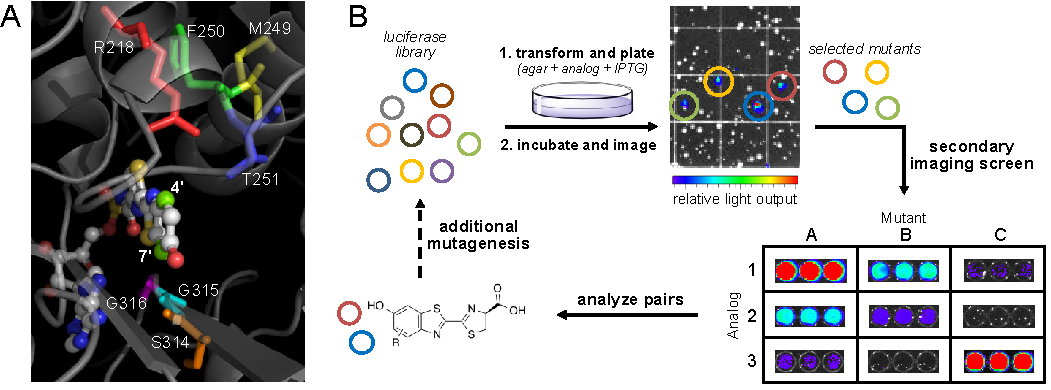
\includegraphics[width= \textwidth]{chapter2/fig3}
\centering
\caption[Generating mutant luciferase libraries and screening for orthogonal pairs]{Generating mutant luciferase libraries and screening for orthogonal pairs. (A) Amino acids targeted for mutagenesis. These residues were
selected based on their proximity to the 4′ and 7′ positions of luciferin. (B) Library screening strategy. An initial on-plate screen identified functional
mutants. These “hits” were subjected to a secondary screen for orthogonality with other mutants and luciferin analogues.}
  \label{fig:residues_screening}
\end{figure}
These selections were partially based on phylogenetic data gathered from across the insect luciferase
family,\cite{RN45, Amaral:2014cz} along with previous biochemical assays: Arg218 is
known to interact with \dluciferin{} and influence the local
structure of the binding pocket;\cite{BRANCHINI:2001gr} F250 lies in close proximity
(∼3 Å) to the benzothiazole ring of \dluciferin{}; T251 has been
shown to potentiate substrate binding;\cite{Branchini:2003kt} residues 314−316 line
a critical edge near the luciferin phenolate and C7′ position.
Mutations at all of these target sites have been shown to perturb \dluciferin{} binding (and thus light emission), while
preserving the overall structural integrity of the enzyme.\cite{Branchini:2007bw, Branchini:2003kt, Viviani:2013ej}
\par
Saturation mutagenesis was used to prepare the desired
libraries. The degree of mutation applied at each residue was
based on the following considerations: sequence conservation
among the insect luciferase family, the identity of the native
residue, and the location of the residue. For example,
nonconserved residues were mutated to a higher degree
compared to conserved residues in the active site. Codon
compression methods were further used to eliminate
redundancies and reduce the number of transformants (Tables
S1 and S2).\cite{Pines:2014he} The final libraries ranged from 19 to 4800
members in size and were constructed using synthetic gene
assembly\cite{Ness:2002cc} in combination with circular polymerase
extension
cloning (CPEC).\cite{Quan:2011fa}
%(Tables S3−S9)
\par
The libraries were screened for orthogonal substrate usage
using a two-tiered approach. Library DNA was first introduced
into bacteria, and the transformants were arrayed across agar
plates containing embedded luciferins (Figure \ref{fig:residues_screening}B). Light-emitting
colonies were easily identified, and in
some cases, the light emission values were on par with native
Fluc and \dluciferin{}. A handful of the
corresponding mutants were sequenced. Some mutations
were observed for multiple analogues, suggesting that they
might be selective for bulky luciferins. Other
mutations were unique to each compound, which is notable,
given the subtle structural differences between some of the
analogues. The number of colonies screened was ∼3× the
calculated diversity for each library.
\par
While initial screens revealed functional mutants (and
quickly culled nonfunctional enzymes), they did not report
on selective substrate usage (i.e., orthogonality). The on-plate
screens also did not control overall expression levels and
differences in compound transport. To address these
parameters, we performed a secondary screen. Colonies
emitting detectable levels of light on-plate were selected and
expanded overnight. These cultures were then lysed and
imaged with analogues. Mutants that provided light emission
on par with native Fluc were identified as bona fide hits and used to create next-generation sequences. This iterative process
was performed to evolve large pools of diverse, but functional,
enzymes. Hits from these subsequent generations were
ultimately tested with all luciferin analogues in secondary
screens.
\par
To mine the entire collection of imaging data for substrateselective
pairs, we first developed a measure of orthogonality
(equation shown in Figure \ref{fig:mining_verifying}A).
\begin{figure}[htbp]
\includegraphics[width= \textwidth]{chapter2/fig4}
\centering
\caption[Analyzing orthogonal enzyme−substrate pairs]{Analyzing orthogonal enzyme−substrate pairs. (A) Representative emission of luciferase mutants screened against a panel of luciferin
analogues. These data were analyzed with a computer algorithm to determine lead mutants with the strongest orthogonality. (B) Purified mutants
exhibit orthogonality. Enzyme (1 μg) was incubated with 100 μM of luciferin analogues, and emission intensities were used to determine the
orthogonality quotient (the ratio of the total flux for the C4/C7 or C7/C4 pairings). The geometric mean is plotted, and the error bars represent the
95\% confidence intervals for n $>$ 4 experiments. (C) Total flux for lead mutants B and C highlights substrate selectivity between C4′ and C7′
sterically modified luciferins. Error bars represent the standard error of the mean for n $>$ 4 experiments.}
  \label{fig:mining_verifying}
\end{figure}
Favorable values are obtained
when two mutants (e.g., A and B) react robustly with unique
substrates (e.g., compounds \cmpd{1} and \cmpd{2}, respectively) in a mutually
exclusive manner. Thus, the more selective a pair of enzymes
for their cognate substrates, the larger the orthogonality rating.
Since the number of potential pairings exceeded 3000 in our
data set, we wrote a computer script to rapidly examine all pairs
in an unbiased fashion. The program iterated through each
possible combination, calculating the corresponding orthogonality
rating. The script ultimately returned a list of pairs ranked
by their potential for orthogonality (and thus utility for
multicomponent imaging).
\par
The top pairs identified by the script exhibited selectivity for
analogues \cmpd{3b} (mutants A and B) and \cmpd{2b}−\cmpd{d} (mutant C). The
magnitude of each mutant’s preference--defined as the
orthogonality quotient--was analyzed. As shown in Figure
\ref{fig:mining_verifying}B and C, mutants A and B exhibited nearly a 100-fold preference for \cmpd{3b} over other analogues, while mutant C strongly favored C7′-modified analogues. Biochemical analyses further indicated that the “brightest”
mutant enzymes were those capable of most efficient substrate
turnover (Table \ref{tb:kinetics}).
\begin{table}
  \caption{Biochemical analyses of orthogonal enzyme−
substrate pairs}
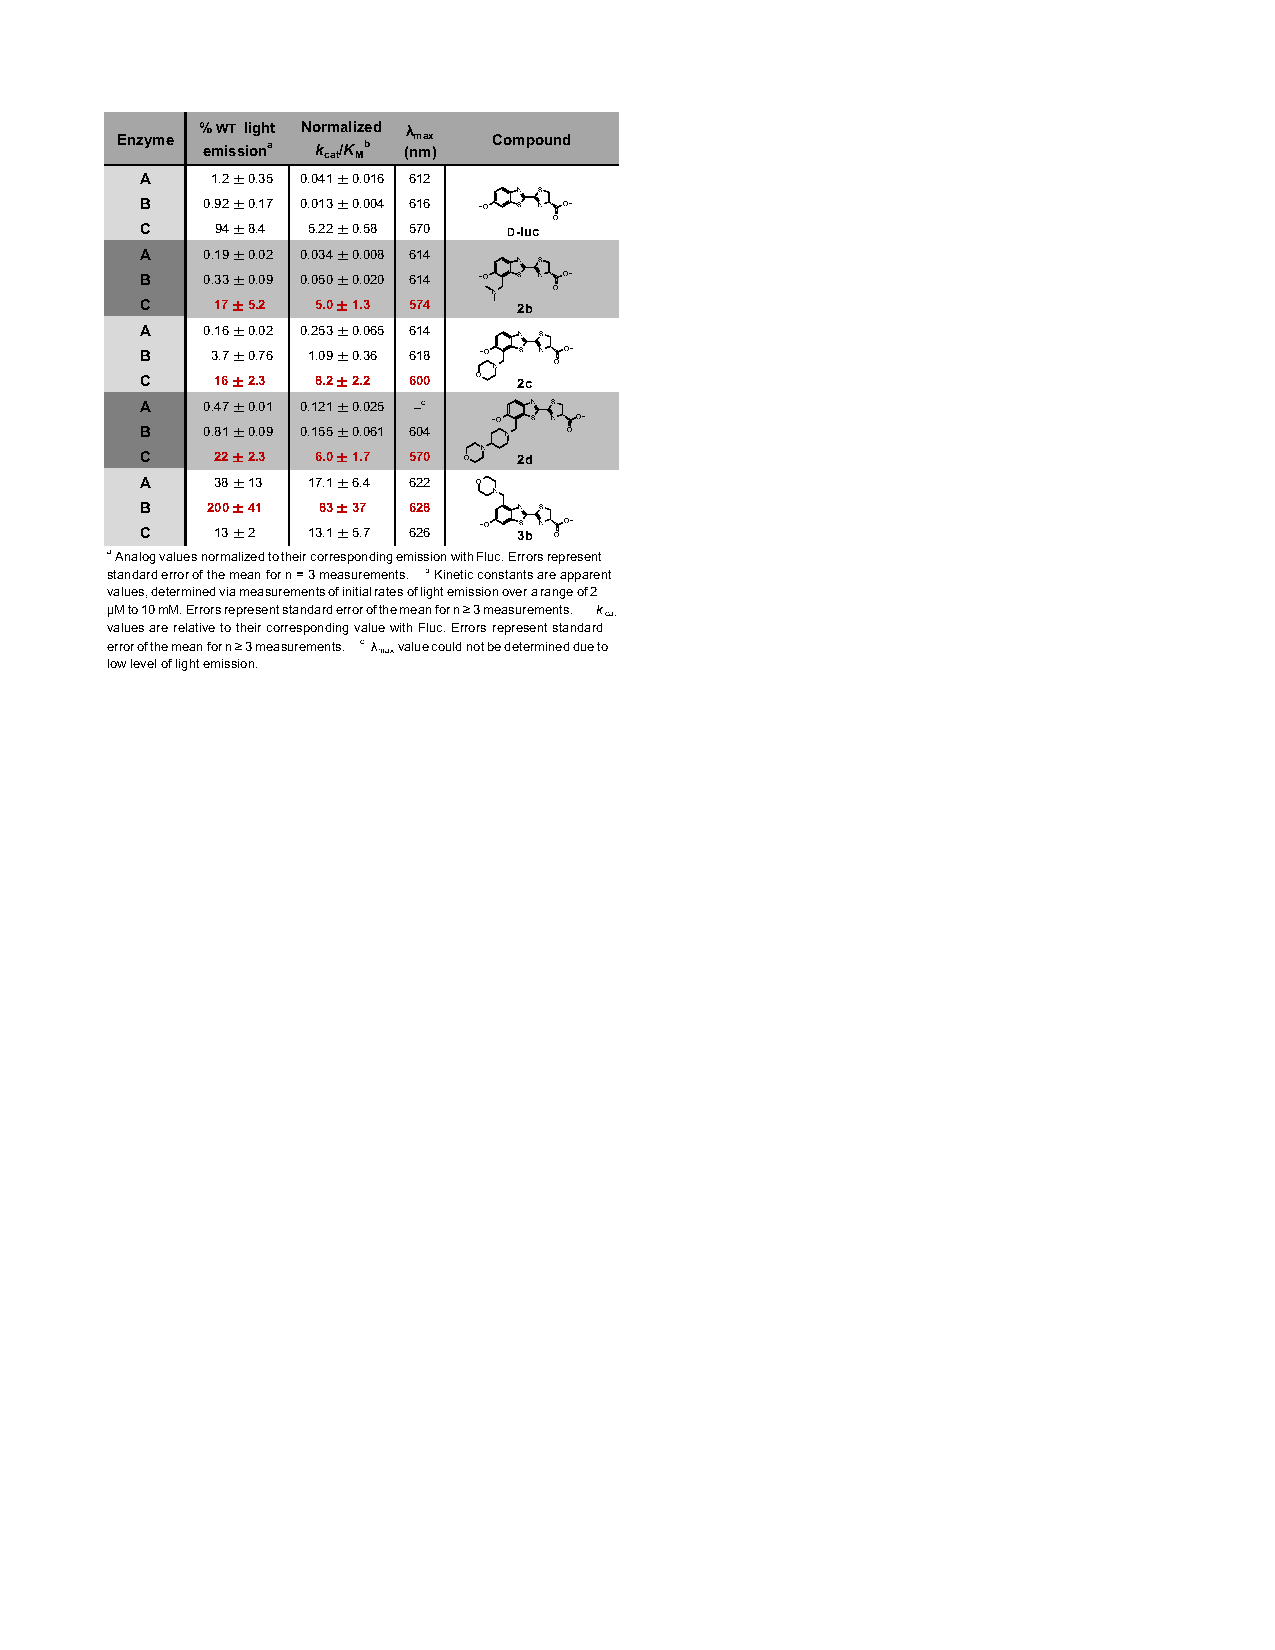
\includegraphics{chapter2/table1}
\centering
  \label{tb:kinetics}
\end{table}

\subsection*{Analyzing the origins of orthogonality}

The identities
of the mutant hits provided some insights into the origins of
substrate orthogonality. Mutant A had a single arginine to
alanine mutation at amino acid 218. Mutant B comprised the
same R218A mutation but harbored additional mutations at
residues 250 (Phe to Met), 314 (Ser to Thr), and 316 (Gly to
Thr). These residues are known to play a role in modulating
binding and interaction with the luciferin substrate. The R218A
mutant is especially interesting, as it is known to greatly reduce
light production and red shift emission with \dluciferin{}.\cite{BRANCHINI:2001gr} It has
been hypothesized that the smaller Ala group allows more
water molecules to access the active site, potentially quenching
light emission.\cite{BRANCHINI:2001gr} The bulky morpholino substituent of \textbf{3b} could
fill this active site void to retain photon production. The third
mutant (mutant C) was more selective for the C7′-modified
luciferins compared to the C4′-modified compound. Mutant C
harbored a single mutation, R218K. R218K may slightly enlarge
the active site of the luciferase. This mutation has also been
shown to boost activity with bulkier cyclic aminoluciferin
analogues.\cite{Harwood:2011gl} The improved selectivity with \textbf{2b−d} could be the
result of active site positioning. The C7′ substituents could
potentially place the luminophore in a more advantageous spot
for light emission.
\par
To delve into the origins of selectivity, we prepared a small
library of additional mutants based on enzyme B (R218A,
F250M, S314T, G316T). R218A seemed critical for discriminating
the regioisomeric compounds, so this residue was held
constant across the series. All possible combinations of the
remaining mutations (F250M, S314T, G316T, or native Fluc
residues) were then allowed. Imaging analyses of these
combinatorial mutants indicated that R218A and F250M
were critical for luciferin discrimination (Figure \ref{fig:muts_vs_cmpds}).
\begin{figure}[htbp]
\includegraphics[width= \textwidth]{chapter2/figS12}
\centering
\caption[Bioluminescent photon production from luciferin analogs with combinatorial enzymes]{Bioluminescent photon production from luciferin analogs with combinatorial enzymes. Combinatorial mutants were prepared, in which R218A was held constant across the library, while the other positions were allowed to code for mutations from mutant B or native Fluc (WT). (A) Luciferin analogs (500 \textmu{}M) or (B) \dluciferin{} were incubated with lysates expressing mutant luciferases or Fluc (WT) in bioluminescence buffer. Images were acquired as described in the Materials and Methods section. Error bars represent the standard error of the mean for n $>$ 4 experiments.}
  \label{fig:muts_vs_cmpds}
\end{figure}
Both mutations should result in a larger active site, but
why they preferentially accommodate \textbf{3b} over other analogues
remains unknown. It is possible that the mutations disrupt
critical binding interactions with the luciferin core, but that
steric appendages (e.g., on the C4′ side) retain sufficient
contacts for subsequent oxidation. Indeed, when \textbf{3b} was
incubated with R218A/F250M, light emission was maintained
(as compared to Fluc, Figure \ref{fig:muts_vs_cmpds}). When \dluciferin{} and the C7′-modified analogues were incubated with this same mutant,
though, light emission was drastically reduced. Interestingly, the
R218A/S314T mutant exhibited an opposite trend in analogue
selectivity: \textbf{2b} was preferred to \textbf{3b} (Figure \ref{fig:muts_vs_cmpds}). Collectively, these results suggest that mutant luciferases can be tuned to
respond to unique substrates. It is also possible that enzyme
orthogonality is most readily achieved not by improving the
utilization of one substrate but by diminishing reactivity with all
other substrates.

\subsection*{Cellular imaging with orthogonal pairs}

As a step
toward multicomponent imaging applications, we evaluated the
orthogonal enzymes and probes in cultured cell models.
Mammalian cell lines (HEK293 and DB7) were engineered
to express orthogonal mutants A−C. %Equivalent expression levels were confirmed using flow cytometry (Figure S14).
Cells
were incubated with analogues \textbf{2b−d} and \textbf{3b}, and photon
outputs were measured. As shown in Figure \ref{fig:in_vitro}, the substrates
were able to cross cell membranes and access the relevant
luciferases, resulting in sustained emission.
\begin{figure}[htbp]
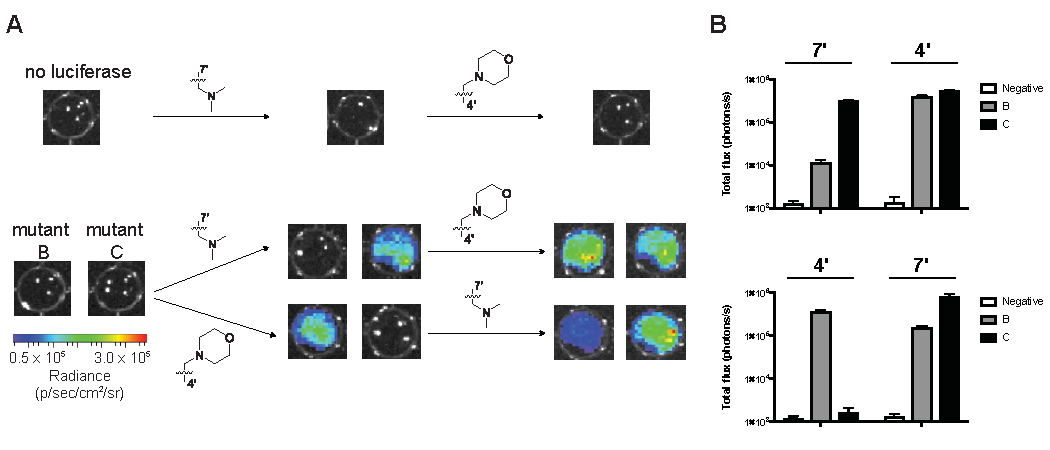
\includegraphics[width= \textwidth]{chapter2/fig5}
\centering
\caption[Imaging cells with orthogonal luciferase−luciferin pairs]{Imaging cells with orthogonal luciferase−luciferin pairs. (A) Mutant luciferase-expressing DB7 cells were plated (1.5 × 10\^{5} cells/well) in
96-well black plates and sequentially incubated with C4′ and C7′ sterically modified luciferins (750 μM). Representative bioluminescence images are
shown. (B) Quantification of the images from (A) after initial substrate addition. Error bars represent the standard error of the mean for experiments
performed in triplicate.}
  \label{fig:in_vitro}
\end{figure}
Photon production
was also confined to cells expressing the complementary
luciferase for each orthogonal luciferin: cells with mutant B
were only visible upon treatment with analogue \textbf{3b}, whereas
cells with mutant C were only visible upon treatment with analogues \textbf{2b−d}.
%(Figures S15−S18).
Importantly, the
orthogonal pairs could also distinguish unique cell types in a
single imaging session. For example, DB7 cells stably expressing
mutant B or C could be readily detected via sequential
administration of the requisite substrates (Figure \ref{fig:in_vitro}).
%Similar
%trends were observed upon imaging HEK293 cells (Figure S19)
%and cocultures (Figure S20).
These data suggest that crossreactivity
between mutants B and C and their non-orthogonal
substrates is minimal.
%The orthogonal pairs also exhibit unique
%emission spectra (Figure S21) that can further enhance some
%multicomponent imaging applications (Figure S22).

\section{Conclusions}

We developed a general strategy to evolve and identify mutant
versions of firefly luciferase that accept distinct, chemically
modified luciferins. Bioluminescence has been largely limited to
visualizing one biological feature at a time, as the most
advantageous luciferases and luciferins for whole-animal
imaging utilize the same substrate and cannot be distinguished
in vivo. To address this void, we generated a family of sterically
modified luciferins that were poor substrates for firefly
luciferase but inherently capable of producing light. Using an
on-plate screen, mutant versions of luciferase were identified
that could also catalyze light emission with other analogues.
Pools of these functional mutants were then further mined for
orthogonal pairs. Some of the mutants could selectively process
individual luciferins both in vitro and in cells, setting the stage
for multicomponent in vivo imaging.
\par
Future studies will be aimed at generating additional
bioluminescent probes with improved brightness and other
optical properties. The enzyme−substrate hits reported here,
while immediately useful, are weaker light emitters than native
bioluminescent systems. Improved light outputs can be
achieved using additional rounds of mutagenesis and screening.
Previous studies have also demonstrated that distant mutations
can profoundly influence the architecture of the luciferase active
site, and these regions will be incorporated into future libraries.
The screening strategy is also broadly applicable to diverse
luciferins, including analogues with altered chromophores that
could provide drastically different colors of light. Our results suggest that enzymes capable of discriminating even subtle
substrate modifications can be readily identified. Such an
outcome bodes well for generating additional orthogonal pairs
and filling a long-standing void in imaging capabilities. We
anticipate that collections of designer luciferins and luciferases
will inspire new discoveries in a variety of disciplines, similar to
how fluorescent protein technology enabled seminal advancements
in numerous fields.

\bibliographystyle{achemso}
\bibliography{thesis2}

%%% Local Variables: ***
%%% mode: latex ***
%%% TeX-master: "thesis.tex" ***
%%% End: ***
